\documentclass[margin=2pt]{standalone}
\usepackage[table]{xcolor}
\usepackage[utf8]{inputenc}
\usepackage[T1]{fontenc}

\usepackage{tikz}
\usepackage{helvet}
\usepackage{amsmath}

\renewcommand\familydefault\sfdefault

% Use \phantom to hide text for exams
\renewcommand{\phantom}{}
\newcommand{\lOS}{\phantom{Operační}\\\phantom{systém}}
\newcommand{\lTaskAssigned}{\phantom{Přiděleno pro}\\\phantom{uživatelskou úlohu}}
\newcommand{\lTaskReal}{\phantom{Paměť skutečně}\\\phantom{použitá pro úlohu}}
\newcommand{\lTaskUnused}{\phantom{Paměť přidělená,}\\\phantom{ale nevyužitá}}

\usetikzlibrary{intersections, shapes.arrows, spath3, shapes.geometric, fit, backgrounds, calc, tikzmark, decorations.pathreplacing, angles, quotes}

\definecolor{themeBlue}{RGB}{1, 103, 143}
\definecolor{themeOrange}{RGB}{221, 109, 16}
\definecolor{themeTeal}{RGB}{18, 54, 69}
\definecolor{themeGrey}{RGB}{120, 121, 124}

\begin{document}
    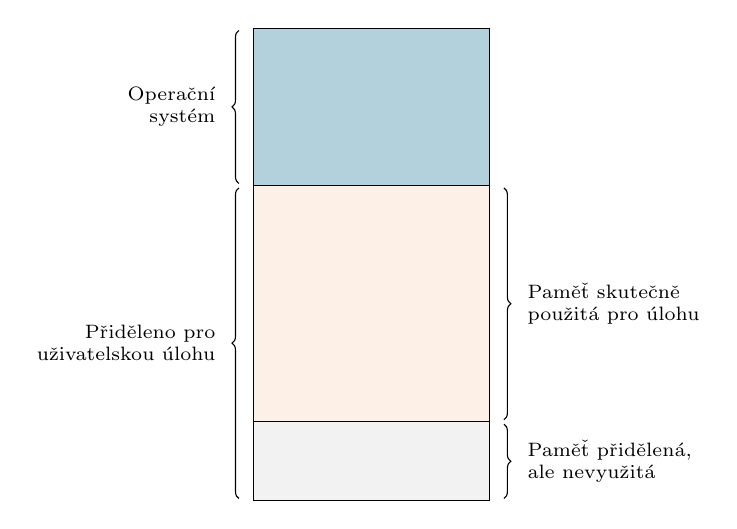
\begin{tikzpicture} [
        width/.style={minimum width=3cm,},
        mem/.style={draw, width, minimum height=9cm, fill=themeGrey!5},
        os/.style={draw, width, anchor=north, minimum height=2cm, fill=themeBlue!30},
        app used/.style={draw, width, anchor=north, minimum height=3cm, fill=themeOrange!10},
        app unused/.style={draw, width, anchor=north, minimum height=1cm, fill=themeGrey!10},
        label left/.style={font=\scriptsize, minimum width=1cm, align=right, left=10pt},
        label right/.style={font=\scriptsize, minimum width=1cm, align=left, right=10pt},
        brace mirror/.style={decoration={brace,mirror,raise=5pt}, decorate},
        brace/.style={decoration={brace,raise=5pt}, decorate}
    ]

    \draw node[os] (os) {};
    \draw (os.south) node[app used, yshift=\pgflinewidth] (app used) {};
    \draw (app used.south) node[app unused, yshift=\pgflinewidth] (app unused) {};

    \draw[brace mirror]  ($ (os.north west) - (0, 1pt) $) -- node[label left] {\lOS} ($ (os.south west) + (0, 1pt) $);
    \draw[brace mirror]  ($ (app used.north west) - (0, 1pt) $) -- node[label left] {\lTaskAssigned} ($ (app unused.south west) + (0, 1pt) $);

    \draw[brace]  ($ (app used.north east) - (0, 1pt) $) -- node[label right] {\lTaskReal} ($ (app used.south east) + (0, 1pt) $);
    \draw[brace]  ($ (app unused.north east) - (0, 1pt) $) -- node[label right] {\lTaskUnused} ($ (app unused.south east) + (0, 1pt) $);

    \end{tikzpicture}
\end{document}